\documentclass[11pt]{article}

\usepackage[a4paper,margin=1in]{geometry}
\usepackage{amsmath,amssymb,amsfonts,mathtools}
\usepackage{bm}
\usepackage{graphicx}
\usepackage{booktabs}
\usepackage{caption}
\usepackage{subcaption}
\usepackage{hyperref}
\usepackage{enumitem}
\usepackage{microtype}
\usepackage{cleveref}

\graphicspath{{report_images/}}
\numberwithin{equation}{section}

\title{Direction D: Inverse Problems and Parameter Identification for Verified Heat Solvers}
\author{Thermalio research notes}
\date{}

\newcommand{\R}{\mathbb{R}}
\newcommand{\dd}{\,\mathrm{d}}
\newcommand{\argmin}{\operatorname*{arg\,min}}
\newcommand{\diag}{\operatorname{diag}}
\newcommand{\norm}[1]{\left\lVert #1 \right\rVert}

\begin{document}
\maketitle

\begin{abstract}
Direction D extends Thermalio from forward verification studies to inverse
thermal-parameter studies.  The implementation keeps the inverse layer thin:
verified forward solvers provide temperature predictions, while a common
observation and residual interface handles sensor sampling, noise, least-squares
optimization, sensitivity diagnostics, discrete adjoints, uncertainty
quantification, regularized perfusion-field recovery, and baseline comparisons
against surrogate and physics-informed neural-network approaches.  This report
summarizes the mathematical processes behind those capabilities and records an
expanded experimental figure set generated under \texttt{report\_images/}.
\end{abstract}

\section{Forward-Inverse Setting}

The main Direction D testbed is the reaction-diffusion/Pennes bioheat model
\begin{equation}
  \partial_t u - \nabla\cdot(\alpha\nabla u) + k u = Q
  \qquad \text{in } \Omega\times(0,T],
  \label{eq:pennes-continuous}
\end{equation}
with temperature $u(\bm{x},t)$, thermal diffusivity $\alpha$, perfusion or
linear reaction coefficient $k$, and source term $Q$.  In the implemented
studies, synthetic observations are generated by the trusted finite-volume
forward map
\begin{equation}
  \mathcal{F}(\bm{\theta}) =
  \left[u_h(\bm{\theta};t_1), \ldots, u_h(\bm{\theta};t_m)\right],
  \label{eq:forward-map}
\end{equation}
where $\bm{\theta}$ may be a scalar perfusion, a vector of parameters such as
$(\alpha,k)$, or coefficients describing a spatially varying perfusion field.
The observation model is
\begin{equation}
  \bm{y} = \mathcal{H}\mathcal{F}(\bm{\theta}_\star) + \bm{\eta},
  \qquad
  \bm{\eta}\sim \mathcal{N}(0,\Sigma_\eta),
  \label{eq:observation-model}
\end{equation}
where $\mathcal{H}$ selects sparse sensors and observation times, and
$\bm{\theta}_\star$ is the known synthetic truth used for verification.

\begin{figure}[t]
  \centering
  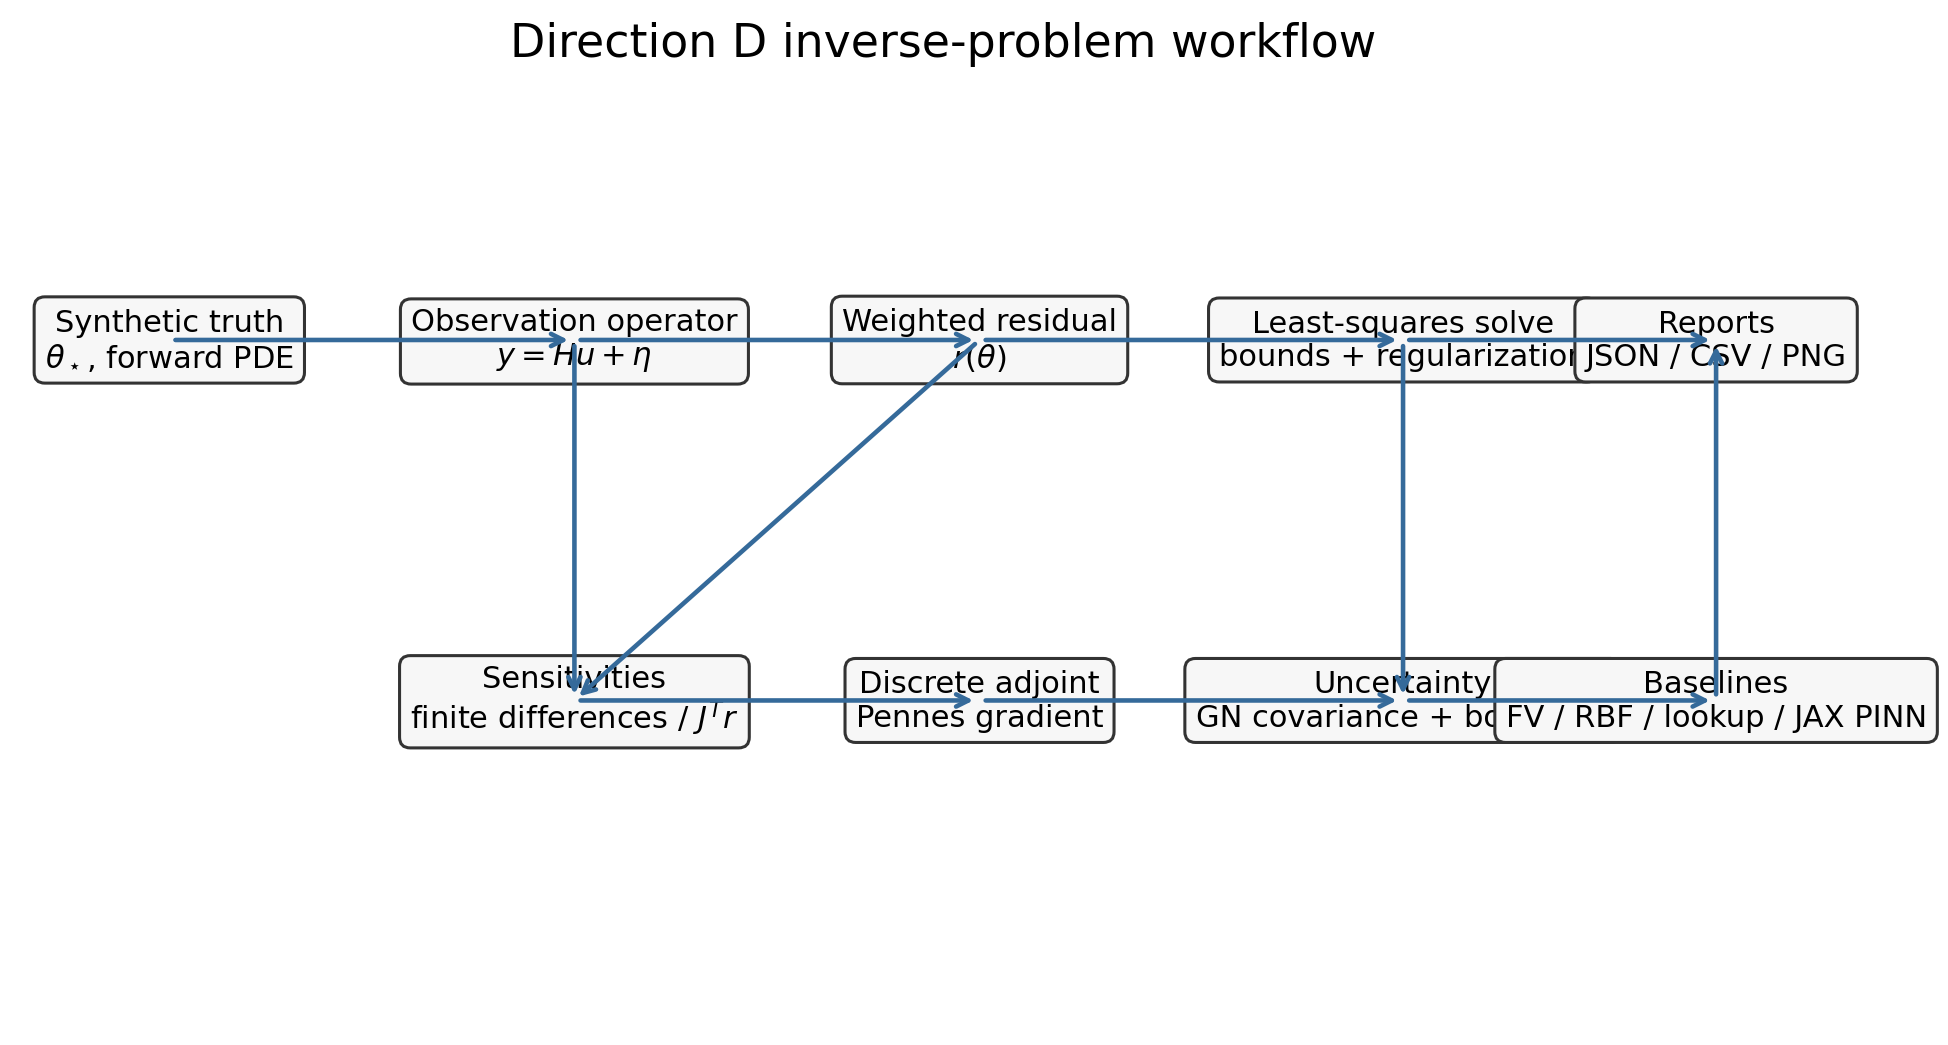
\includegraphics[width=\linewidth]{direction_d_inverse_workflow.png}
  \caption{Functional workflow of the Direction D inverse-problem layer. The verified forward model generates synthetic data; sparse observations define the residual; optimization, sensitivities, adjoints, uncertainty estimates, and baseline comparisons all operate on the same residual contract.}\label{fig:direction-d-workflow}

\end{figure}

\section{Observation Operators and Weighted Residuals}

The sparse/multi-time observation utility implements a discrete sampling
operator.  If $U\in\R^{n_t\times n_s}$ stores a sequence of state snapshots,
sensor indices $S=\{s_1,\ldots,s_p\}$ and time indices
$T=\{\tau_1,\ldots,\tau_q\}$ define
\begin{equation}
  \mathcal{H}(U) =
  \left[
    U_{\tau_1,s_1},\ldots,U_{\tau_1,s_p},
    U_{\tau_2,s_1},\ldots,U_{\tau_q,s_p}
  \right]^T.
  \label{eq:sparse-observation}
\end{equation}
Weights are applied as square roots so that each residual remains compatible
with a standard least-squares norm:
\begin{equation}
  \bm{r}(\bm{\theta}) =
  W^{1/2}\left(\mathcal{H}\mathcal{F}(\bm{\theta})-\bm{y}\right),
  \qquad W=\diag(w_1,\ldots,w_n).
  \label{eq:weighted-residual}
\end{equation}
This form allows quadrature weights, sensor confidence weights, and unweighted
sensor stacks to use the same objective.

\section{Scalar and Vector Parameter Estimation}

The core inverse objective is the bound-constrained nonlinear least-squares
problem
\begin{equation}
  \widehat{\bm{\theta}}
  =
  \argmin_{\bm{\ell}\leq\bm{\theta}\leq\bm{u}}
  \frac{1}{2}\norm{\bm{r}(\bm{\theta})}_2^2.
  \label{eq:least-squares}
\end{equation}
The scalar wrapper specializes \cref{eq:least-squares} to a single unknown, for
example perfusion $k$.  The vector form supports multi-parameter recovery, such
as joint diffusivity and perfusion estimation.  The implementation delegates the
nonlinear solve to SciPy's trust-region least-squares optimizer, while keeping
all residual construction local and explicit.

Identifiability scans evaluate the same cost on a prescribed grid:
\begin{equation}
  \Phi(\bm{\theta}_i) =
  \frac{1}{2}\norm{\bm{r}(\bm{\theta}_i)}_2^2.
  \label{eq:identifiability-scan}
\end{equation}
For one parameter this produces a cost curve; for two parameters it produces a
Cartesian cost surface.  These scans are not the optimizer itself.  They are
diagnostics for curvature, local uniqueness, and parameter tradeoff.

\begin{figure}[t]
  \centering
  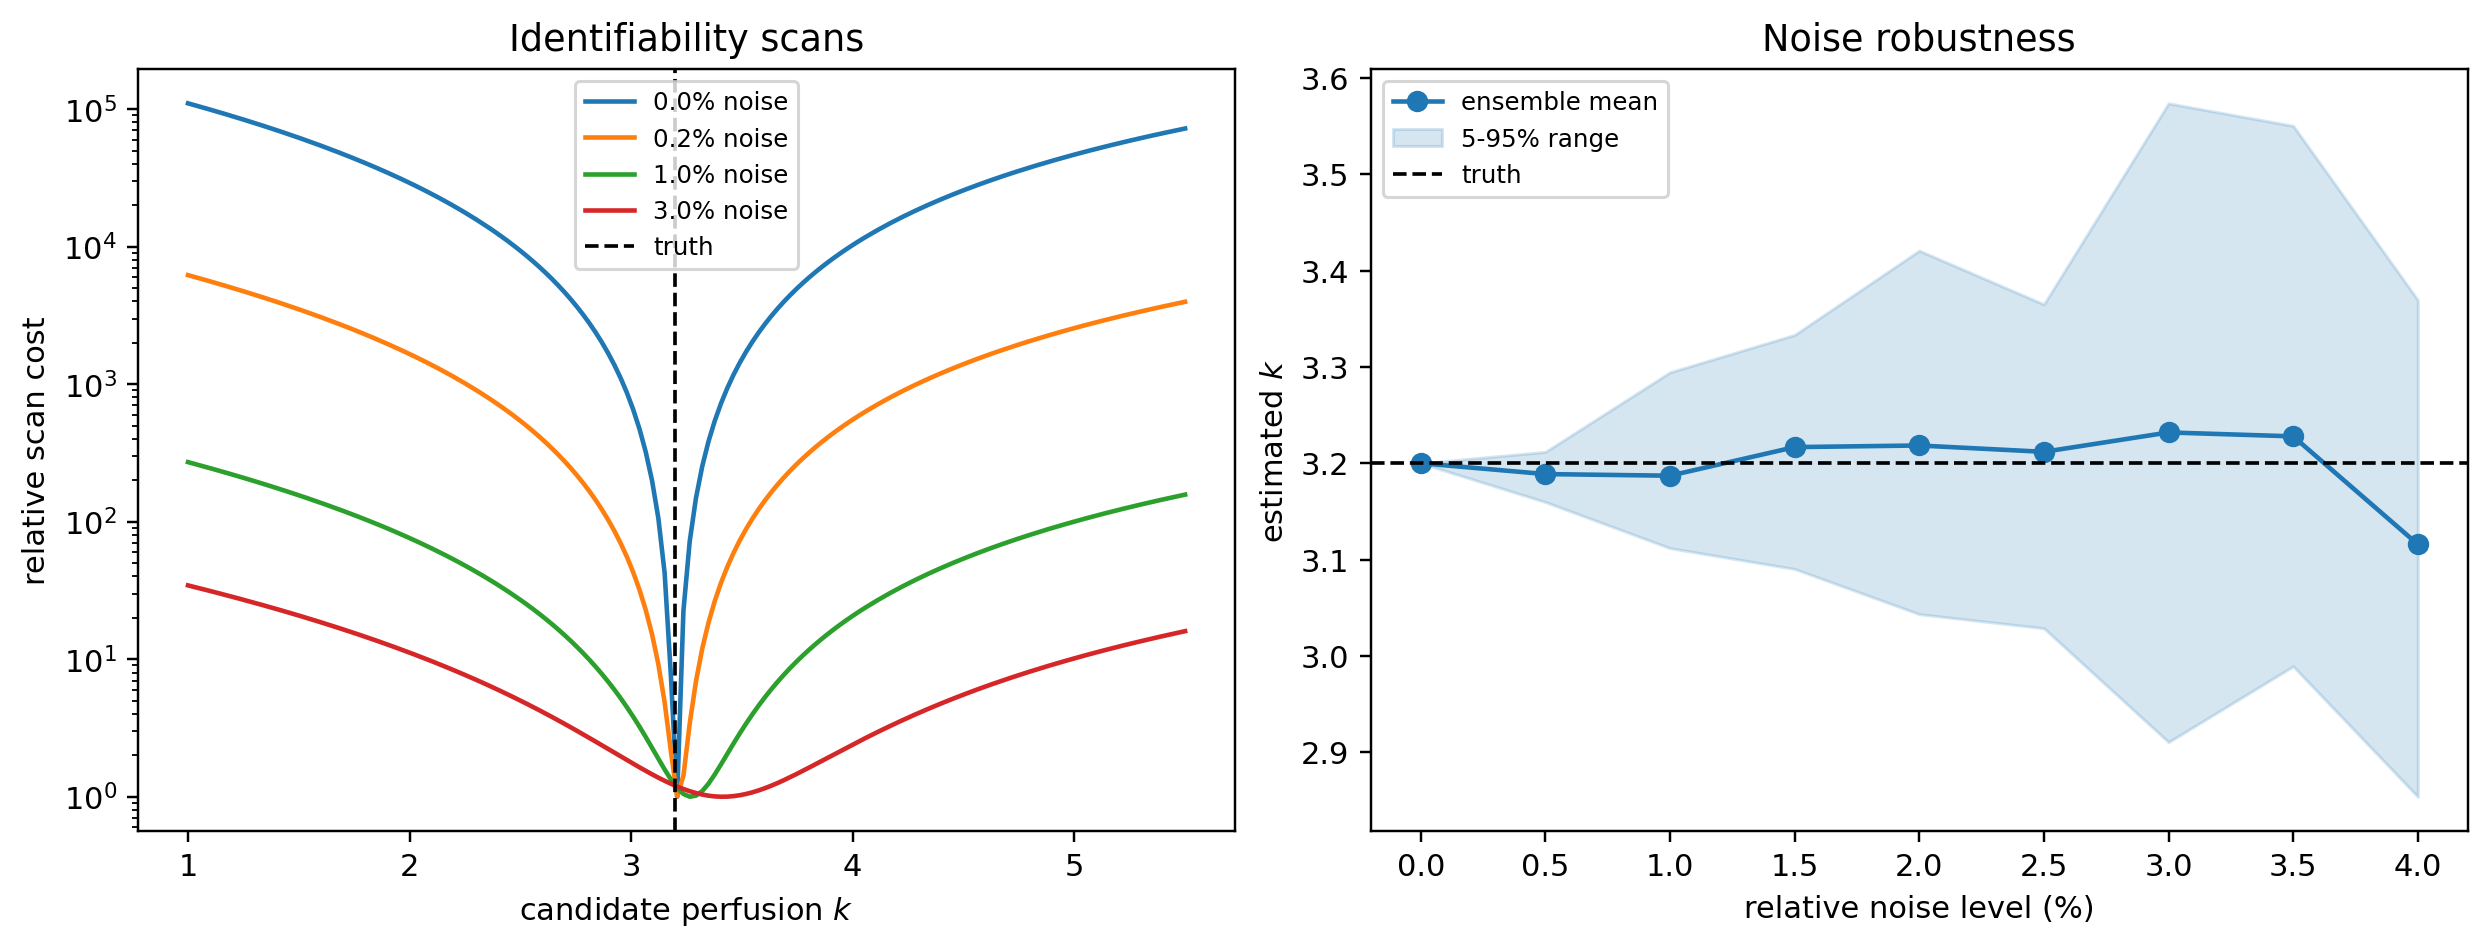
\includegraphics[width=\linewidth]{scalar_identifiability_noise.png}
  \caption{Scalar Pennes perfusion recovery under increasing observation noise. Left: scan costs retain a clear minimum near the truth for low-to-moderate noise. Right: repeated noisy inversions show the estimator remains centered near the truth while the 5--95\% uncertainty band expands with noise.}\label{fig:scalar-identifiability-noise}

\end{figure}

\begin{figure}[t]
  \centering
  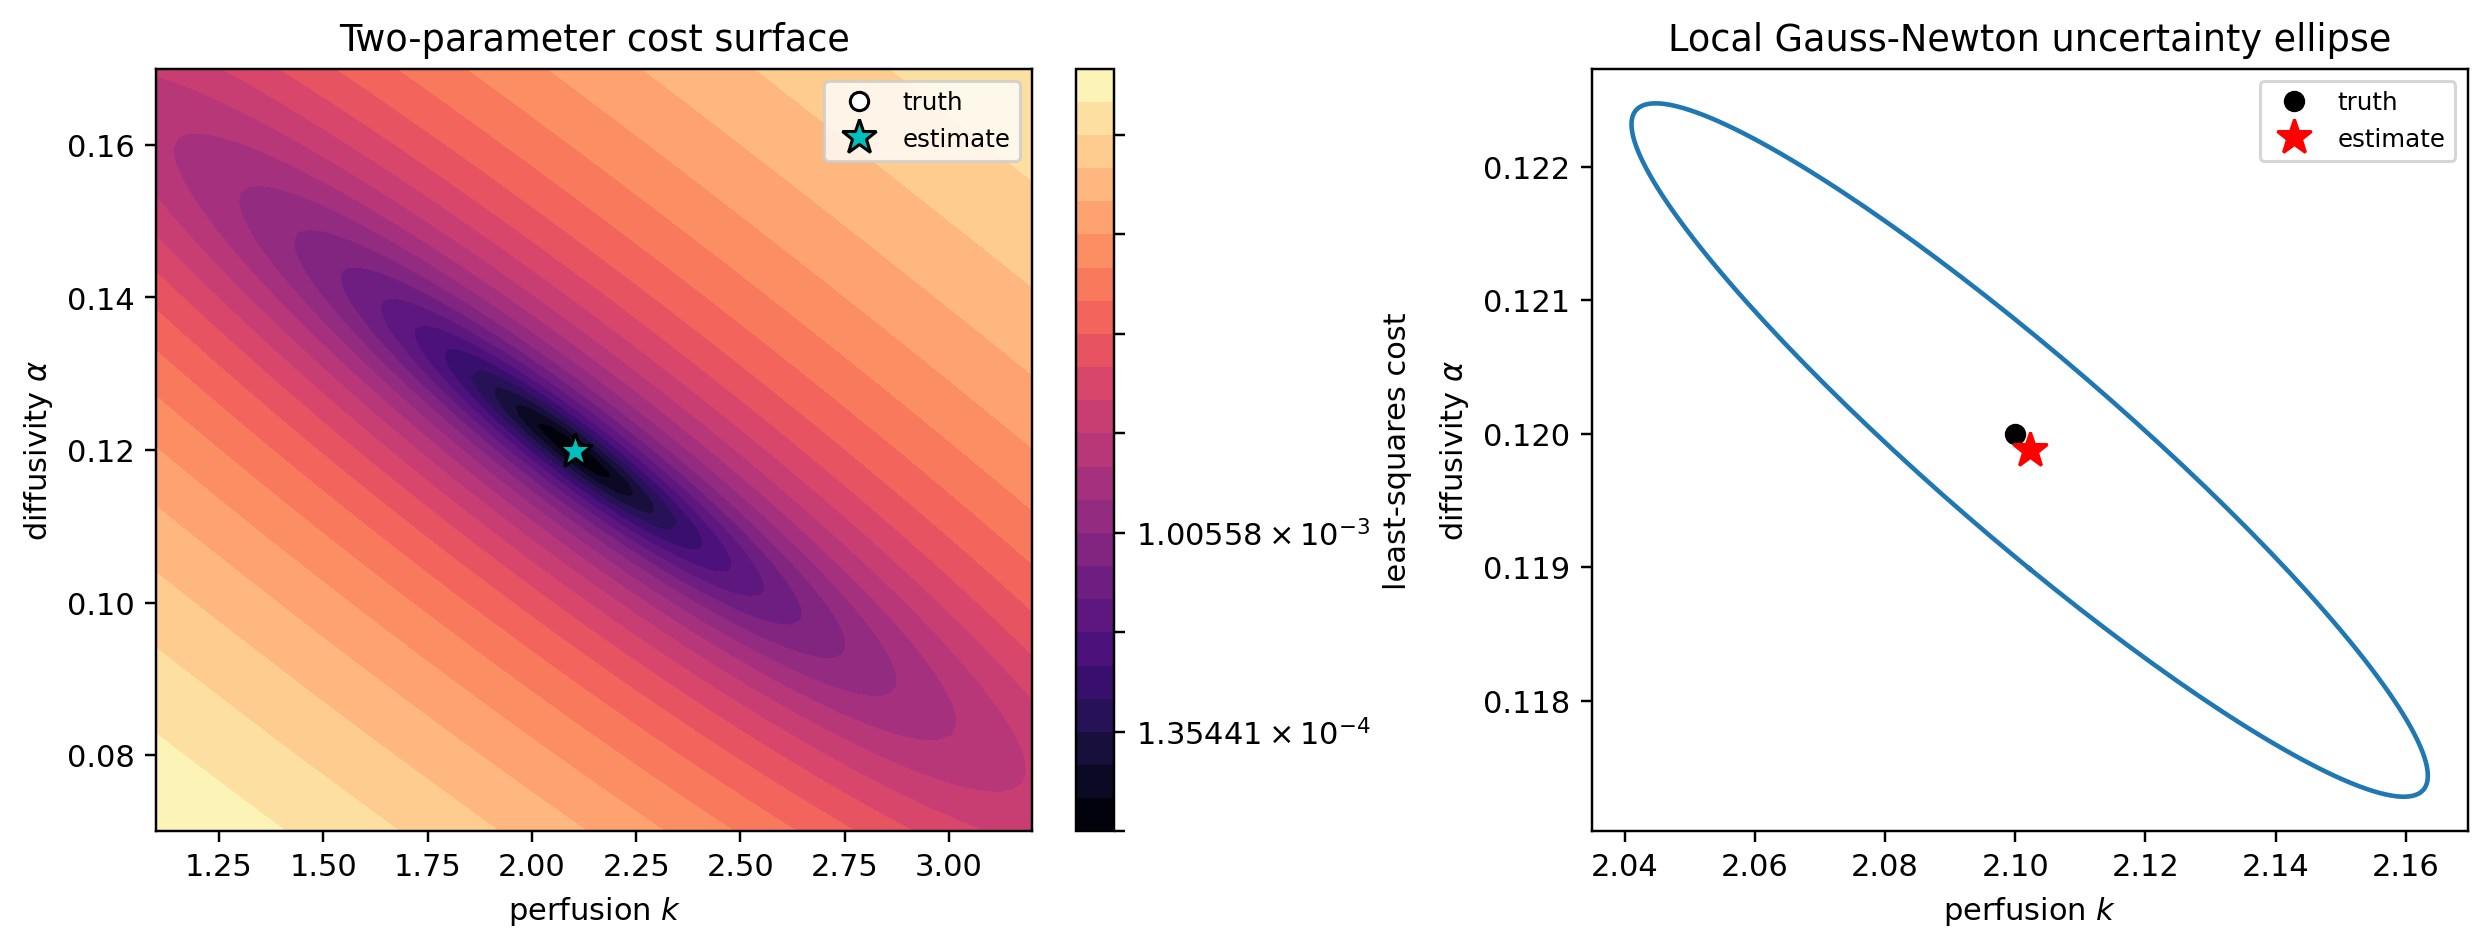
\includegraphics[width=\linewidth]{multi_parameter_identifiability.png}
  \caption{Joint diffusivity-perfusion identification for a two-mode synthetic Pennes response. The cost surface shows the local basin used by the optimizer, while the Gauss-Newton covariance ellipse summarizes parameter coupling around the recovered point.}\label{fig:multi-parameter-identifiability}

\end{figure}

\section{Regularization}

Ill-posed or underdetermined inverse problems are stabilized by appending a
regularization residual to the data residual:
\begin{equation}
  \bm{R}(\bm{\theta})
  =
  \begin{bmatrix}
    \bm{r}_{\mathrm{data}}(\bm{\theta})\\
    \bm{r}_{\mathrm{reg}}(\bm{\theta})
  \end{bmatrix}.
  \label{eq:stacked-residual}
\end{equation}
For a prior vector $\bm{\theta}_0$, component scale $\bm{s}$, and strength
$\lambda\geq 0$, the prior residual is
\begin{equation}
  \bm{r}_{\mathrm{reg}}(\bm{\theta})
  =
  \sqrt{\lambda}\,
  \frac{\bm{\theta}-\bm{\theta}_0}{\bm{s}}.
  \label{eq:prior-regularization}
\end{equation}
The matrix form uses a linear operator $L$ and target $\bm{b}$:
\begin{equation}
  \bm{r}_{\mathrm{reg}}(\bm{\theta})
  =
  \sqrt{\lambda}\,
  S^{-1}\left(L\bm{\theta}-\bm{b}\right).
  \label{eq:matrix-regularization}
\end{equation}
In the field-inversion runner, $L$ can be a pairwise-difference matrix between
Gaussian-basis coefficients.  This penalizes rough coefficient patterns without
requiring a full cellwise unknown at every mesh cell.

\begin{figure}[t]
  \centering
  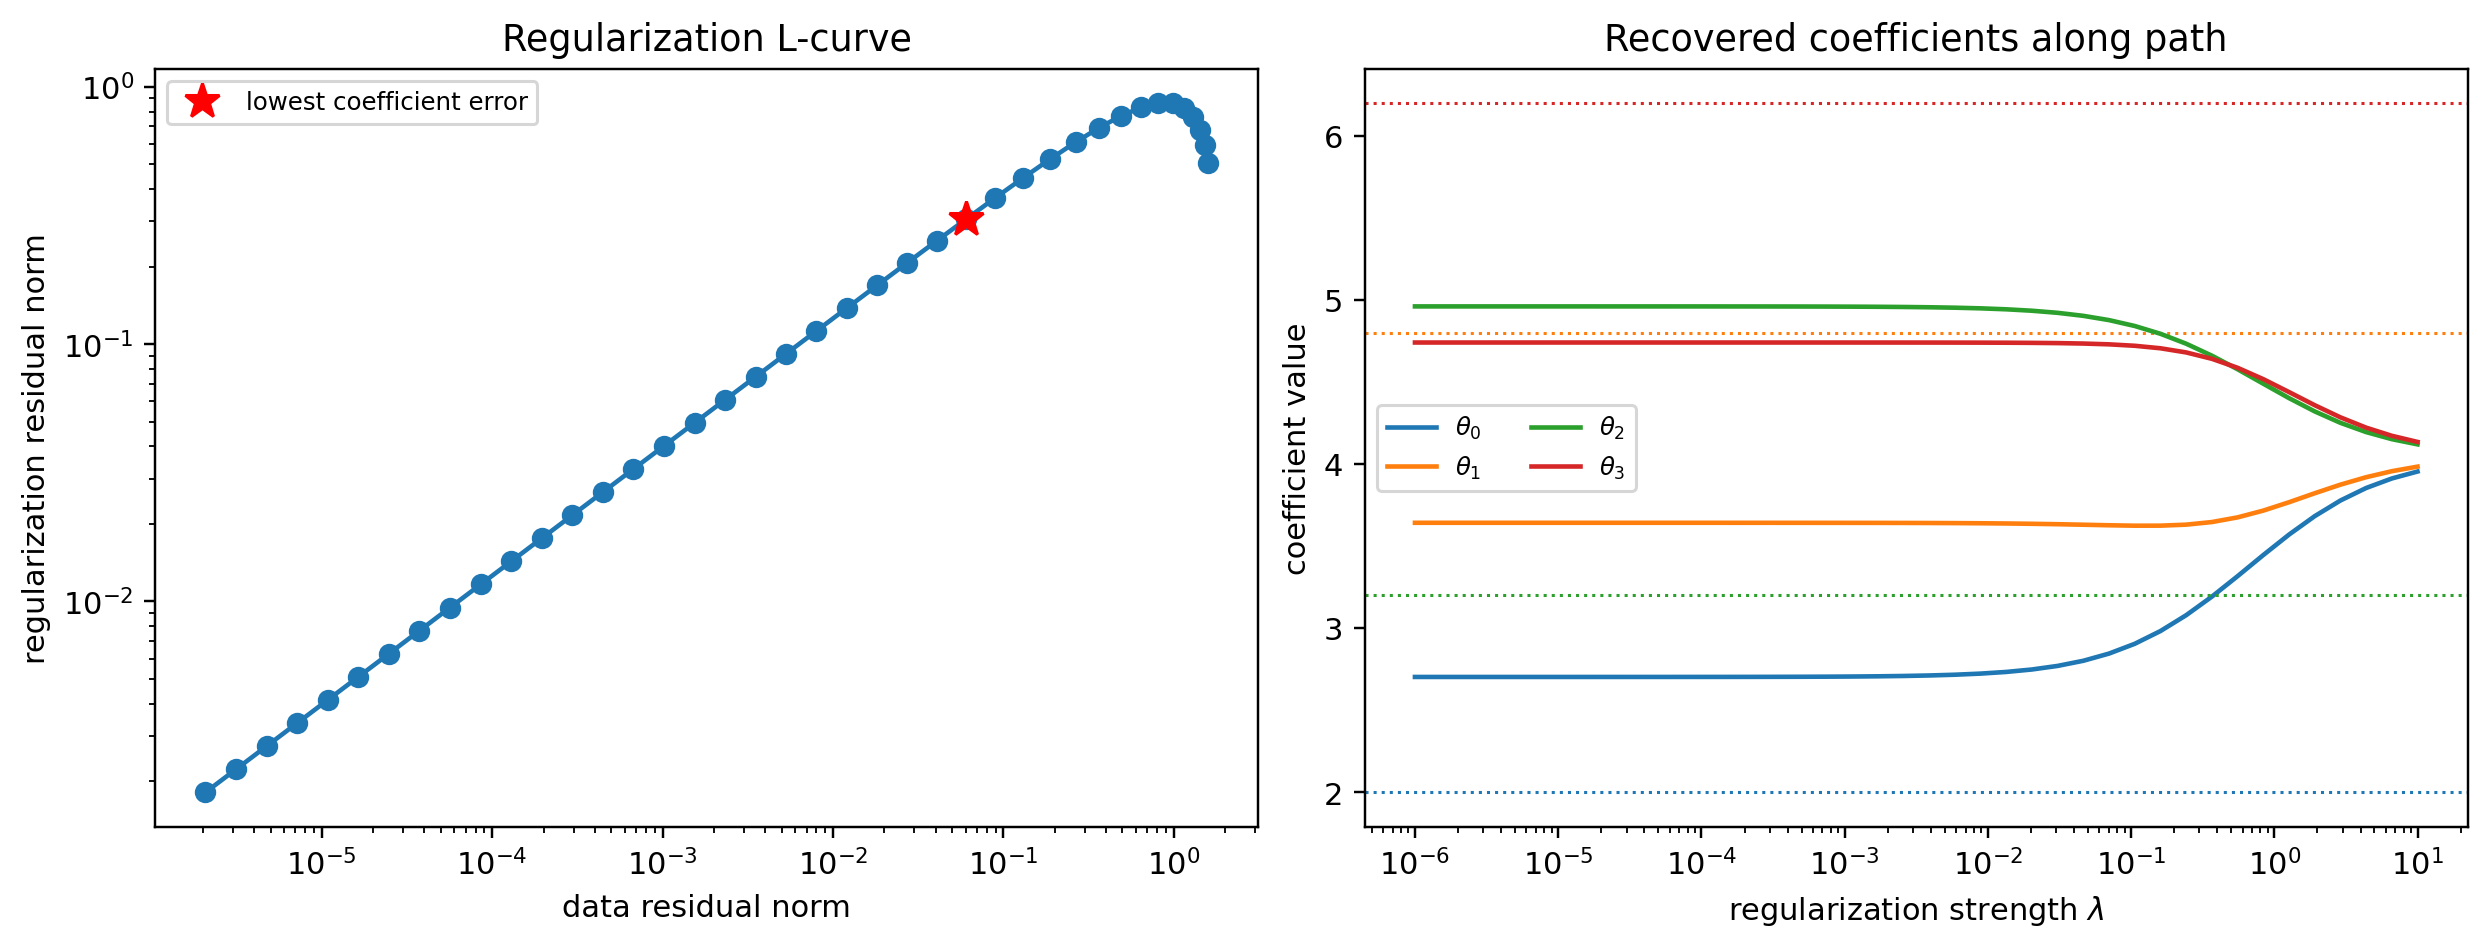
\includegraphics[width=\linewidth]{regularization_path_expanded.png}
  \caption{Regularization-path diagnostic for an underdetermined coefficient inverse problem. The L-curve exposes the data-fit versus prior-penalty tradeoff, while the coefficient traces show how stronger Tikhonov regularization damps non-identifiable directions.}\label{fig:regularization-path-expanded}

\end{figure}

\section{Sensitivity Diagnostics}

For a vector-valued forward map $f(\bm{\theta})$, the finite-difference
Jacobian approximates
\begin{equation}
  J_{ij} =
  \frac{\partial f_i}{\partial \theta_j}.
  \label{eq:jacobian-definition}
\end{equation}
The central-difference stencil used away from bounds is
\begin{equation}
  J_{\cdot j}
  \approx
  \frac{
    f(\bm{\theta}+h_j\bm{e}_j) -
    f(\bm{\theta}-h_j\bm{e}_j)
  }{2h_j}.
  \label{eq:central-difference}
\end{equation}
Near a parameter bound, the implementation falls back to a one-sided difference
that remains inside the feasible interval.  Given residual $\bm{r}$, the
least-squares gradient is the adjoint product
\begin{equation}
  \nabla_\theta \left(\frac{1}{2}\norm{\bm{r}}_2^2\right)
  =
  J_r^T\bm{r},
  \label{eq:jt-r}
\end{equation}
where $J_r$ is the Jacobian of the residual.  The function
\texttt{least\_squares\_gradient} exposes this product directly for diagnostic
and verification use.

\section{Discrete Pennes Adjoint}

Finite differences are simple but expensive because every parameter direction
requires additional forward solves.  Direction D therefore implements a
discrete adjoint for scalar Pennes perfusion in the backward-Euler solver.  Let
$M=\diag(|C_i|)$ be the mass matrix, $A$ the finite-volume diffusion operator,
$R(k)$ the reaction matrix, and $K(k)=A+R(k)$.  One forward step is
\begin{equation}
  B(k)u^n = M u^{n-1} + \Delta t\,\bm{q}^n,
  \qquad
  B(k)=M+\Delta t\,K(k).
  \label{eq:be-forward}
\end{equation}
For observations at selected steps, define
\begin{equation}
  \mathcal{J}(k)
  =
  \frac{1}{2}
  \sum_{n\in\mathcal{T}_{obs}}
  \norm{W_n^{1/2}\left(H_nu^n-\bm{y}^n\right)}_2^2.
  \label{eq:adjoint-objective}
\end{equation}
The backward recursion solves
\begin{equation}
  B(k)^T\lambda^n
  =
  H_n^TW_n(H_nu^n-\bm{y}^n)
  +
  M\lambda^{n+1},
  \label{eq:adjoint-recursion}
\end{equation}
with zero observation contribution when $n$ is not observed.  Since
$\partial R/\partial k$ is the diagonal cell-volume reaction contribution, the
scalar gradient accumulated by the implementation is
\begin{equation}
  \frac{\dd \mathcal{J}}{\dd k}
  =
  -\Delta t
  \sum_{n=1}^{N}
  \left(\lambda^n\right)^T
  M u^n,
  \label{eq:pennes-adjoint-gradient}
\end{equation}
with boundary entries excluded where Dirichlet conditions overwrite the state.
The tests compare \cref{eq:pennes-adjoint-gradient} against central finite
differences of the fully discrete objective.

\section{Uncertainty Quantification}

Direction D includes two uncertainty diagnostics.  The local Gaussian
approximation uses the Gauss-Newton covariance
\begin{equation}
  C_\theta
  \approx
  \widehat{\sigma}^2
  \left(J_r^TJ_r\right)^+,
  \label{eq:gn-covariance}
\end{equation}
where $(\cdot)^+$ denotes the pseudo-inverse and $\widehat{\sigma}^2$ is a
residual-variance estimate.  For confidence level $1-\alpha_c$, the normal
interval for parameter $\theta_i$ is
\begin{equation}
  \widehat{\theta}_i
  \pm
  z_{1-\alpha_c/2}\sqrt{(C_\theta)_{ii}}.
  \label{eq:confidence-interval}
\end{equation}
The bootstrap/noise ensemble repeatedly perturbs observations and re-solves the
inverse problem:
\begin{equation}
  \widehat{\bm{\theta}}^{(b)}
  =
  \argmin_{\bm{\theta}}
  \frac{1}{2}
  \norm{
    \mathcal{H}\mathcal{F}(\bm{\theta})
    -
    \left(\bm{y}+\bm{\eta}^{(b)}\right)
  }_2^2.
  \label{eq:bootstrap}
\end{equation}
Sample quantiles of $\{\widehat{\bm{\theta}}^{(b)}\}$ give a non-asymptotic
interval estimate.

\begin{figure}[t]
  \centering
  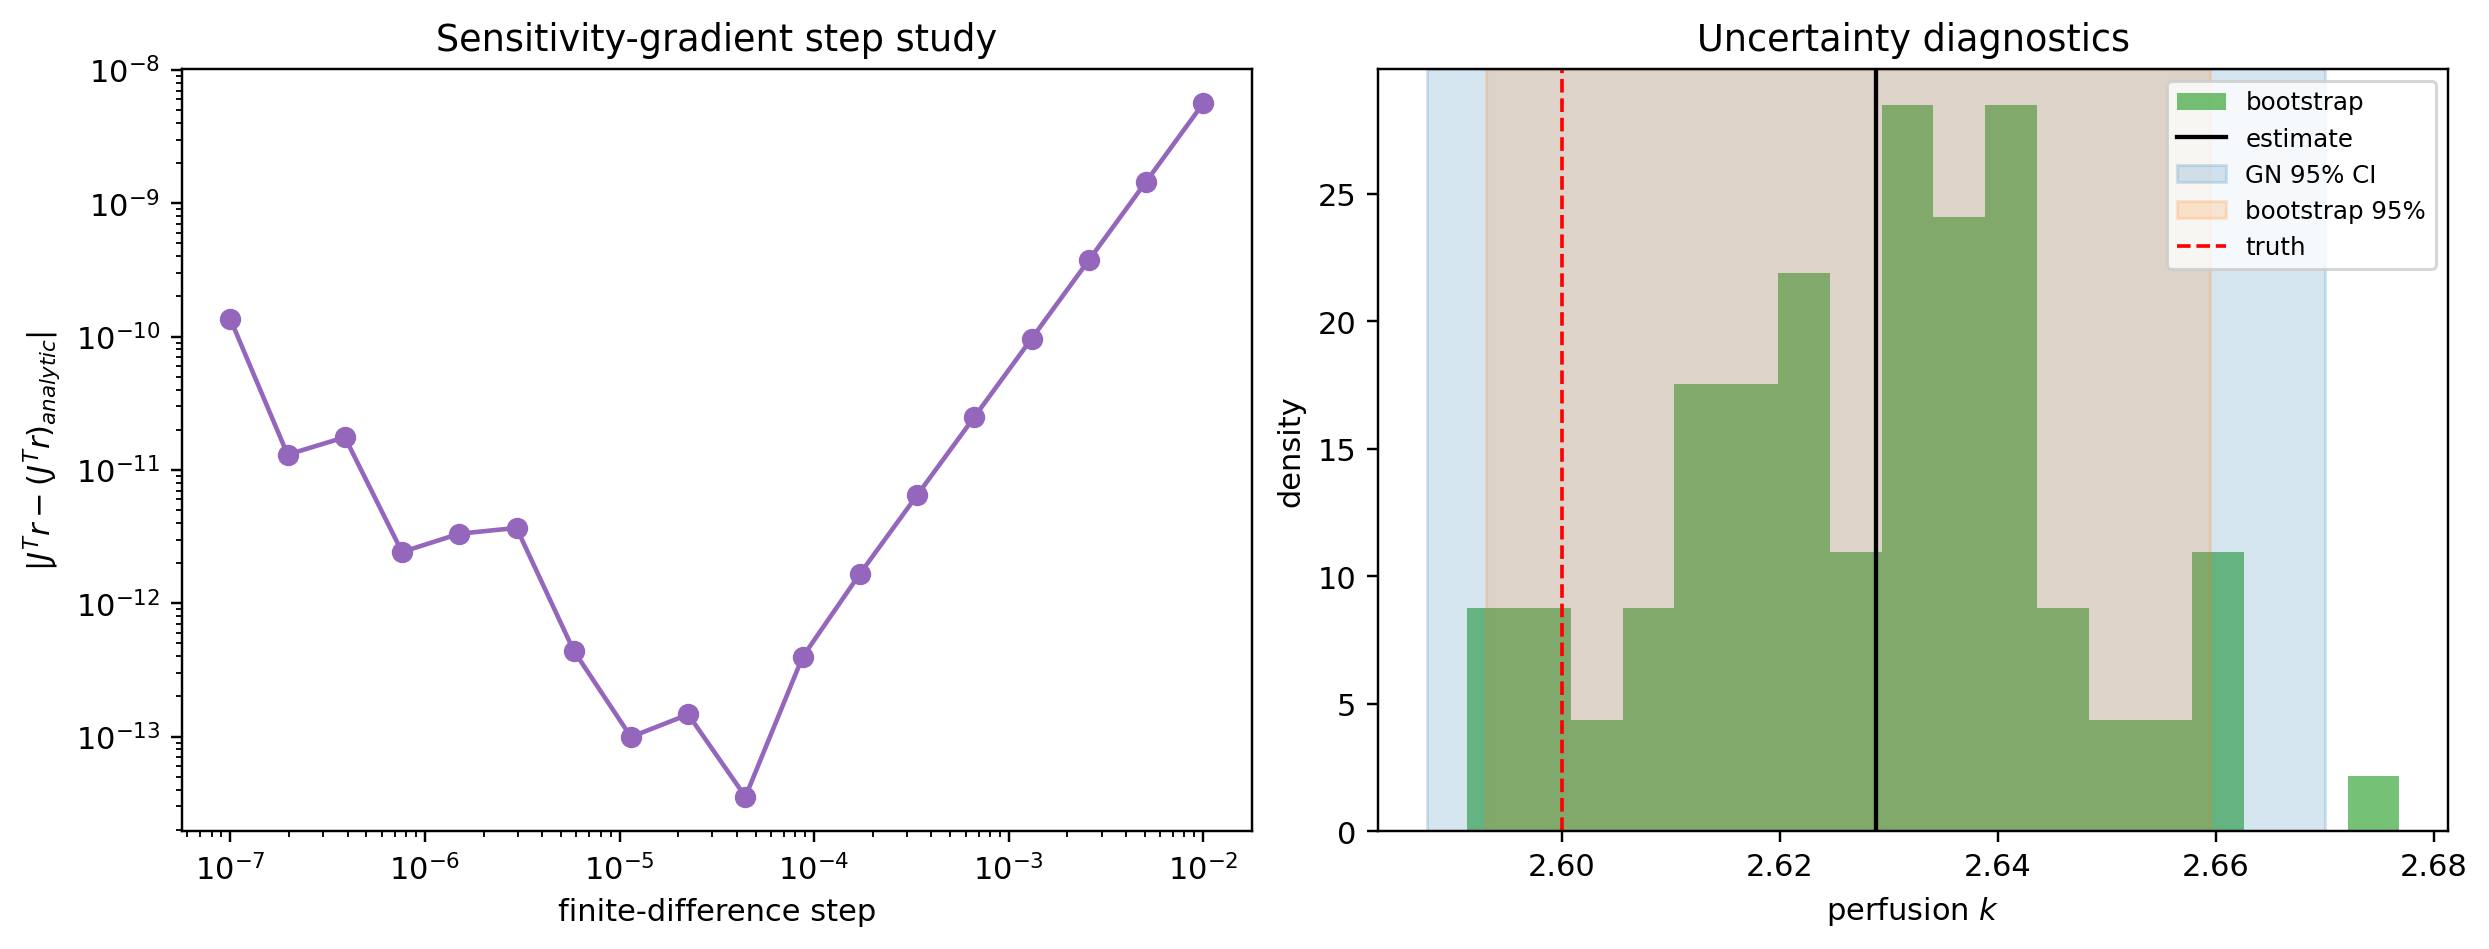
\includegraphics[width=\linewidth]{sensitivity_uq_diagnostics.png}
  \caption{Sensitivity and uncertainty diagnostics. The finite-difference gradient shows the expected step-size tradeoff, and the fitted perfusion uncertainty is summarized with both a local Gauss-Newton 95\% confidence interval and a bootstrap/noise-ensemble 95\% interval.}\label{fig:sensitivity-uq-diagnostics}

\end{figure}

\section{Regularized Perfusion-Field Inversion}

The field-inversion runner represents a spatially varying perfusion coefficient
by a normalized Gaussian radial basis:
\begin{equation}
  k(\bm{x};\bm{c})
  =
  \sum_{\ell=1}^{p}
  c_\ell \phi_\ell(\bm{x}),
  \qquad
  \phi_\ell(\bm{x})
  =
  \frac{
    \exp\left(-\norm{\bm{x}-\bm{\mu}_\ell}^2/(2\rho^2)\right)
  }{
    \sum_{j=1}^{p}
    \exp\left(-\norm{\bm{x}-\bm{\mu}_j}^2/(2\rho^2)\right)
  }.
  \label{eq:gaussian-field}
\end{equation}
This reduces a field inverse problem to a low-dimensional coefficient inverse
problem.  The study solves
\begin{equation}
  \widehat{\bm{c}}
  =
  \argmin_{\bm{0}\leq\bm{c}\leq\bm{c}_{max}}
  \frac{1}{2}
  \norm{
    \mathcal{H}\mathcal{F}(\bm{c})-\bm{y}
  }_2^2
  +
  \frac{\lambda}{2}
  \norm{L\bm{c}}_2^2,
  \label{eq:field-inverse}
\end{equation}
where $L$ is a smoothness operator on the basis coefficients.  The report
artifacts include coefficient tables, field plots, and RMSE metrics.

\begin{figure}[t]
  \centering
  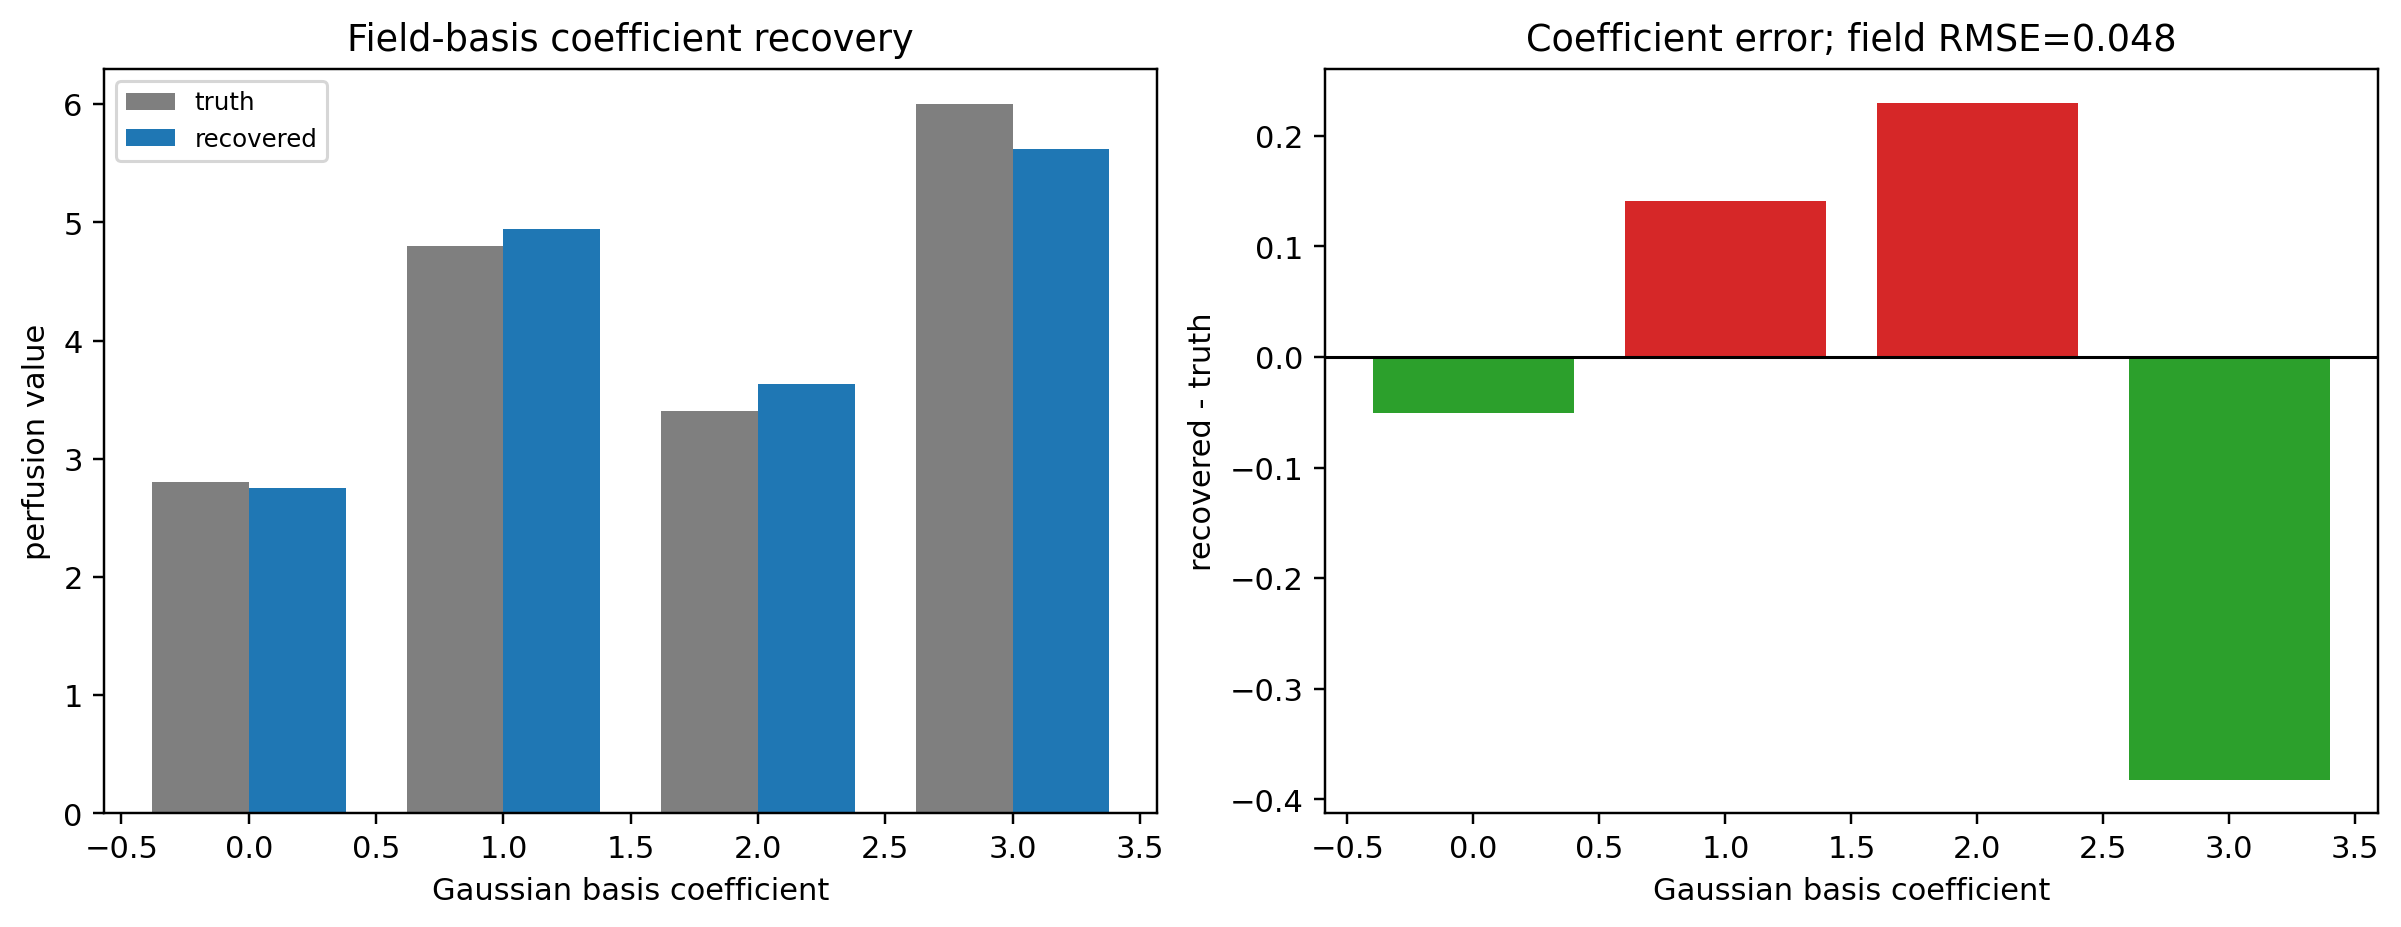
\includegraphics[width=\linewidth]{field_inversion_coefficients.png}
  \caption{Regularized Pennes perfusion-field inversion summarized in coefficient space. The normalized Gaussian basis recovers the main spatial trend while the error panel identifies which basis locations dominate the remaining field RMSE.}\label{fig:field-inversion-coefficients}

\end{figure}

\section{Baseline and PINN Comparisons}

The baseline-comparison runner uses a common row schema with fields
\texttt{name}, \texttt{kind}, \texttt{estimate}, and \texttt{predicted}.  Each
candidate method is scored by the same residual metrics:
\begin{equation}
  e_{abs}=|\widehat{k}-k_\star|,
  \qquad
  e_{rel}=\frac{|\widehat{k}-k_\star|}{|k_\star|},
  \qquad
  \rho=\frac{\norm{\widehat{\bm{y}}-\bm{y}}_2}{\norm{\bm{y}}_2}.
  \label{eq:baseline-metrics}
\end{equation}
The dependency-light baselines are:
\begin{enumerate}[label=\arabic*.]
  \item trusted finite-volume inverse solve,
  \item RBF-ridge surrogate trained on finite-volume parameter sweeps,
  \item nearest training-grid lookup.
\end{enumerate}
The optional JAX PINN adapter trains a neural representation
$u_\omega(x,y,t)$ and a bounded perfusion parameter $k_\zeta$ using the loss
\begin{align}
  \mathcal{L}(\omega,\zeta)
  &=
  w_d
  \frac{1}{N_d}
  \sum_i
  |u_\omega(\bm{x}_i,t_i)-y_i|^2
  +
  w_p
  \frac{1}{N_p}
  \sum_j
  |\mathcal{R}_p[u_\omega,k_\zeta](\bm{x}_j,t_j)|^2
  \notag\\
  &\quad+
  w_0
  \frac{1}{N_0}
  \sum_j
  |u_\omega(\bm{x}_j,0)-u_0(\bm{x}_j)|^2
  +
  w_b
  \frac{1}{N_b}
  \sum_j
  |u_\omega(\bm{x}_j,t_j)-g(\bm{x}_j,t_j)|^2,
  \label{eq:pinn-loss}
\end{align}
where
\begin{equation}
  \mathcal{R}_p[u,k]
  =
  \partial_t u
  -
  \alpha(\partial_{xx}u+\partial_{yy}u)
  +
  k u.
  \label{eq:pinn-residual}
\end{equation}
Automatic differentiation supplies the PINN derivatives.  The current JAX run
is a progress diagnostic rather than a fully tuned benchmark, but it is already
compatible with the same reporting schema as the finite-volume and surrogate
baselines.

\begin{figure}[t]
  \centering
  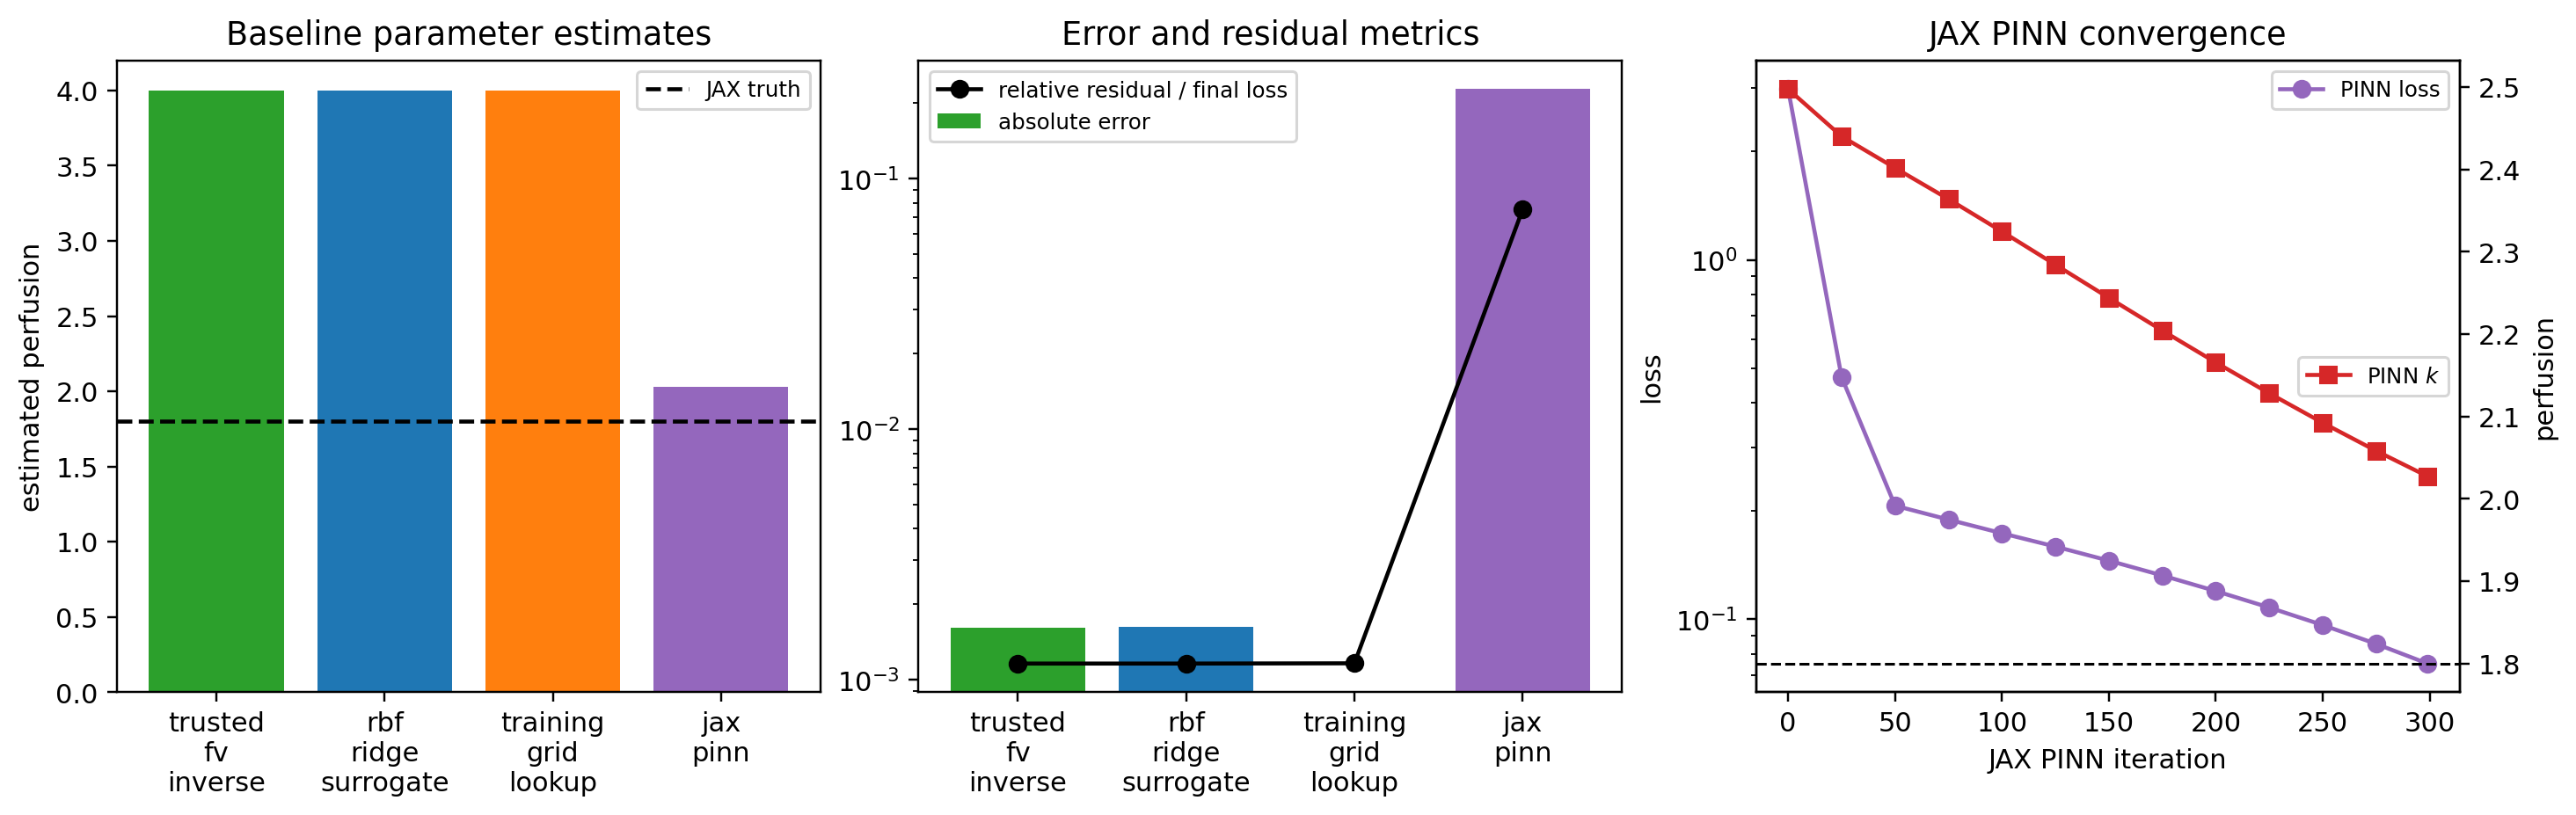
\includegraphics[width=\linewidth]{baseline_comparison_expanded.png}
  \caption{Expanded baseline comparison. Trusted finite-volume inversion, an RBF-ridge surrogate, a training-grid lookup, and the optional JAX PINN are placed on a common estimate/error schema; the right panel shows the JAX PINN loss and perfusion trajectory.}\label{fig:baseline-comparison-expanded}

\end{figure}

\section{Implementation and Reproducibility}

The primary implementation lives in \texttt{heat\_solver/inverse.py}.  Optional
JAX functionality is isolated in \texttt{heat\_solver/pinn\_jax.py} so importing
Thermalio does not require JAX.  Unit tests in \texttt{tests/test\_inverse.py}
cover residual validation, sparse observations, scalar and vector recovery,
finite-difference sensitivities, adjoint-gradient agreement, regularization,
field inversion, and ML-baseline report writing.  Tests in
\texttt{tests/test\_pinn\_jax.py} check lazy optional imports and execute the
JAX backend when \texttt{jax} and \texttt{jaxlib} are available.

The expanded report figures were generated by
\begin{verbatim}
MPLCONFIGDIR=/tmp/matplotlib \
python report_images/generate_direction_d_report_images.py
\end{verbatim}
Each generated PNG has a matching \texttt{*.caption.tex} file in
\texttt{report\_images/}.  The report includes those caption snippets directly,
so changes to figure captions remain colocated with the images.

\section{Summary}

Direction D turns verified heat solvers into a reproducible inverse-problem
testbed.  Its central mathematical idea is a common residual contract:
forward-model predictions are sampled by an observation operator, weighted into
a least-squares residual, and then reused by optimizers, scans, sensitivities,
adjoints, uncertainty tools, regularized field inversions, and baseline
comparisons.  This design keeps the forward physics trusted and explicit while
allowing inverse-method experiments to grow around the same verification
surface.

\end{document}
